\section{Task 2: Reverse engineering the RF protocol} \label{ch:pentesting:rf-reverse-engineering}
This section covers the process of reverse-engineering the RF protocol, via captured RF signals. This included mainly trying to demodulate the signals into binary data and then analyzing the contents.

\subsubsection{Background}
The system in question uses RF signals to wirelessly communicate across the devices. These radio waves are used to transfer binary data, ones and zeroes, between each device. Transferring binary data over radio waves is done by a process called modulation \cite{rf-modulation}. Digital modulation, e.g modulating binary data, is a whole field of study in itself, and that this is only a brief overview covering the basics of modulation.

There are three primary simple ways of modulating a binary signal: Amplitude- (ASK), Frequency- (FSK), and Phase- (PSK) shift keying. They each produce a distinct waveform, which can easily be visually identified. This is shown in figure \ref{fig:digital-modulation}.
\begin{figure}[!ht]
    \centering
    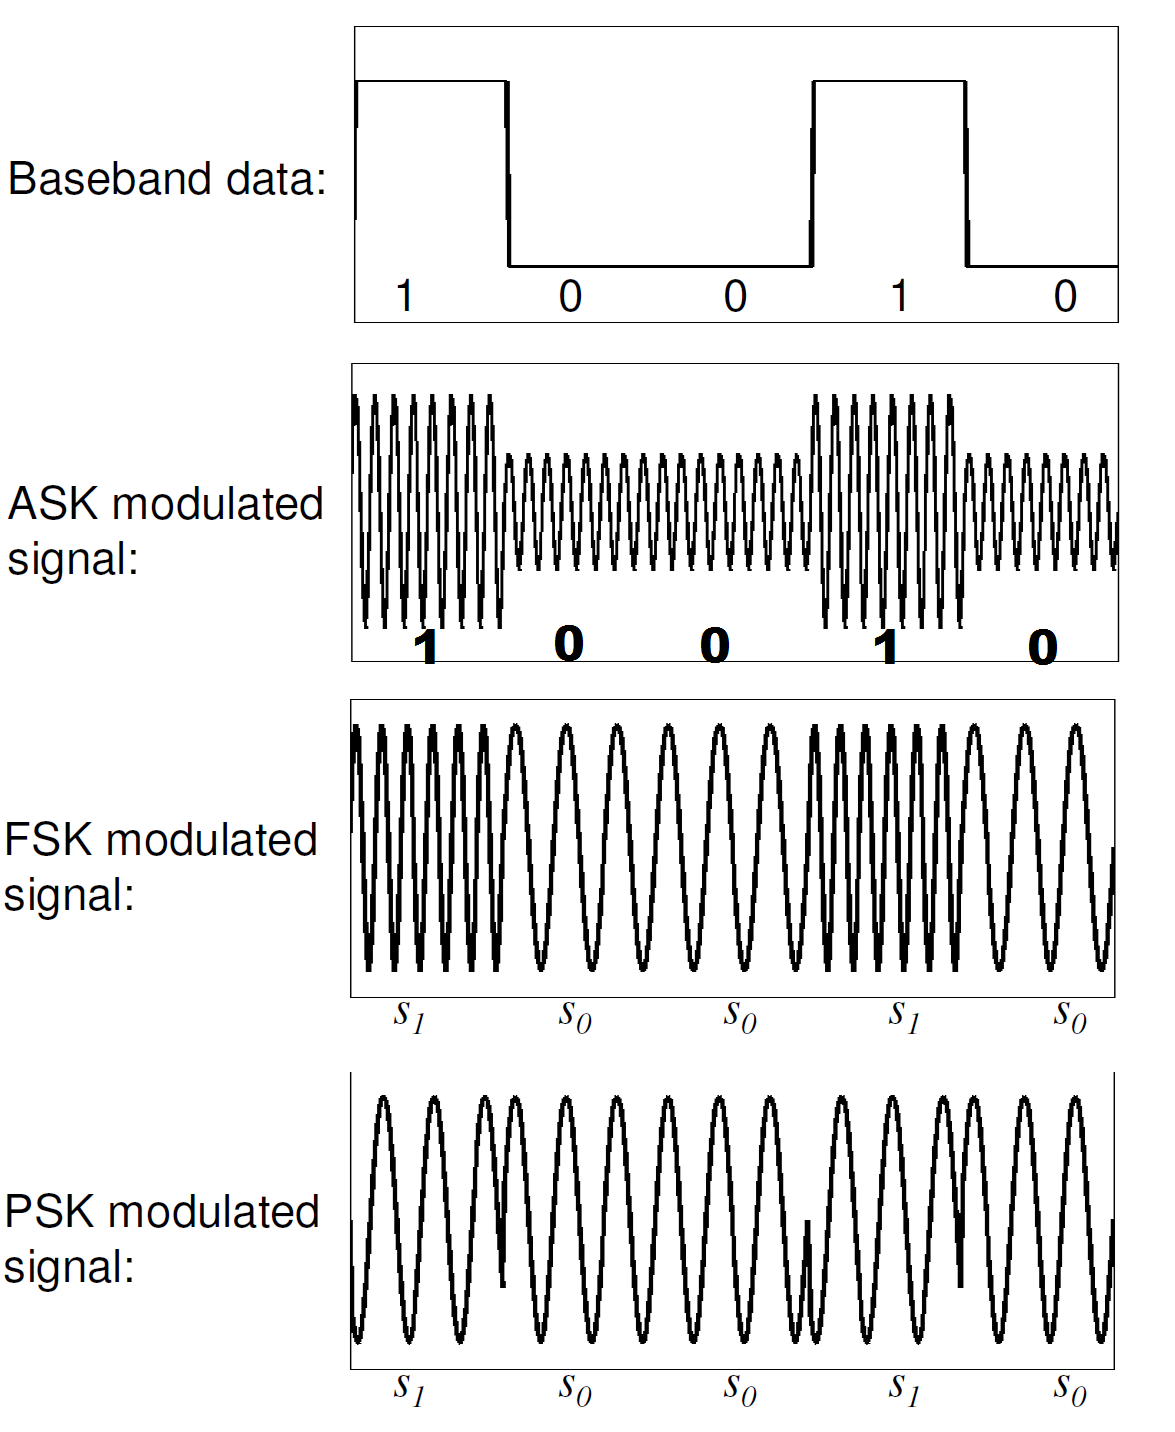
\includegraphics[width=0.5\textwidth]{images/6-pentesting/digital-modulation.png}
    \caption{The three primary techniques for digital modulation.}
    \label{fig:digital-modulation}
\end{figure}

Each technique uses a different property of the sinusoidal wave to encode a zero and one respectively. \gls{ASK} uses the amplitude of the wave, where a higher amplitude usually encodes a \texttt{1} and a lower amplitude a \texttt{0}. The frequency and phase of the wave is kept constant. \gls{FSK}, on the other hand, keeps both amplitude and phase constant. Instead two different frequencies are shifted between to differentiate between a \texttt{0} or \texttt{1}. Lastly, \gls{PSK} uses a phase-shift to differentiate between the two symbols. There are many much more complicated techniques to more efficiently encode a binary signal in radio waves, combining these techniques \cite{rf-modulation}. This can allow for much more information-dense modulation schemes, however, these are considered outside the scope of this thesis.

Conversely, \textit{demodulation} is the process of converting a modulated signal back into the original binary data. In most real-world applications of RF communication this is done directly in hardware, using specialized radio receivers and circuitry to automatically convert the signal back into binary data \cite{rf-modulation}. Often this hardware also implements error correction, noise filtering, and other techniques to increase reliability of the communication, as interference and other disturbances are unavoidable in the real world. Figure \ref{fig:bfsk-demodulator} shows a very simplified circuit that implements binary FSK (BFSK) demodulation, e.g FSK modulation using two parameter frequencies.
\begin{figure}[!ht]
    \centering
    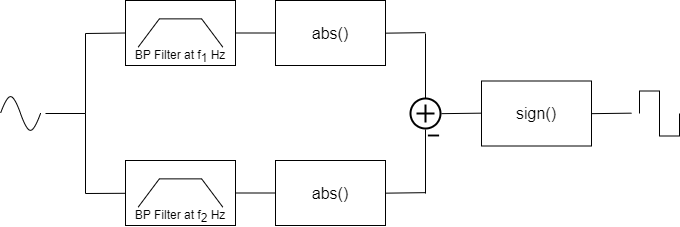
\includegraphics[width=0.8\textwidth]{images/6-pentesting/bfsk-demodulator.png}
    \caption{A simplified BFSK demodulating circuit.}
    \label{fig:bfsk-demodulator}
\end{figure}

Given a BFSK signal, modulated using the frequencies $f_1$ and $f_2$, the circuit does the following. First, the signal is split and passed into two band-pass filters, tuned to the two respective parameter frequencies. Then the absolute value is applied to the signals, one of them is inverted, and they are added together. Lastly, to convert the result into the final binary wave, the signal is passed to the $sign()$ function. This circuit was inspired by material from the course \textit{EE123 Digital Signal Processing} at Berkeley EECS\footnotelink{https://sites.google.com/berkeley.edu/ee123-sp20/labs}{2021-05-18}, specifically Lab 4 which covers FSK demodulation. Demodulation can of course also be done in software, but doing so in real-time is quite CPU-intensive and consequently a lot less energy efficient. Moreover, for each modulation type, there are several tuneable parameters that are hardcoded in the hardware demodulation chip, such as the frequencies of the FSK modulation, which during reverse engineering have to be figured out \cite{hacking-the-iot-talk, rf-exploitation-talk}, as covered in section \ref{ch:related-work:hacking-iot} and \ref{ch:related-work:rf-exploit}.

\subsubsection{Method}
Initially, signals were captured according to the method described in the method part of section \ref{ch:pentesting:replay:method}, using \gls{URH}. Carefully inspecting the signals in URH, as shown in figure \ref{fig:zoomed-in-signal}, one can see that clearly \gls{FSK} modulation is used to modulate the signal. This conclusion is corroborated by the official user manual submitted to the FCC \cite{hsgw-user-manual}, as well as official test documentation submitted to the \textit{Ministry of Internal Affairs and Communications} (MIC) in Japan \cite{mic-test-report}, in which the modulation type is specified to be FSK.

Furthermore, one of \gls{URH}'s key features is automatic demodulation \cite{urh-paper}. This was tested on all captured signals. However, it was unfortunately continuously unsuccessful to automatically find the correct parameters of the modulation. Instead, the signals were demodulated \textit{by hand} using the open-source audio processing tool \textit{Audacity}\footnotelink{https://www.audacityteam.org}{2021-05-17}. The method to do this was inspired by the circuit shown in figure \ref{fig:bfsk-demodulator}, as well as an excellent tutorial by hobby radio enthusiast Nick Oakman, showing how to demodulate an FSK signal using Audacity \cite{oakman-fsk}. This was done in the following steps:
\begin{enumerate}
    \item The raw signal data, as captured by URH, was imported into Audacity via the menu options \textit{File - Import - Raw Data}. URH saves the signal as raw IQ data of signed 8-bit bytes. By selecting the encoding \textit{Signed 8-bit PCM} with \textit{2 Channels (Stereo)}, the I and Q components of the data get separated and imported into two separate tracks. Using only one of them is enough to extract information in this case. As such the stereo track was split into two mono tracks in Audacity and the second one was then deleted. The rest of the import options do not matter.

    \item Secondly, the center frequency, as perceived by Audacity, was noted. This can be found by the menu options \textit{Analyze - Plot Spectrum}. Note that due to several features like the sample rate not being part of the raw signal data, this frequency might not equal the actual center frequency of \texttt{868.64 MHz}. This frequency was used in the steps below.

    \item A \textit{High-Pass Filter} was applied to the first track, and a \textit{Low-Pass Filter} to the second, with the \textit{Roll-off} value set to \texttt{48 dB}. The former essentially map a higher frequency to a higher amplitude in the output wave, and the latter does the opposite.

    \item Using Audacity's scripting language Nyquist\footnotelink{https://www.audacityteam.org/about/nyquist}{2021-05-17} the absolute value was applied to each track. The short Nyquist program \mintinline[style=emacs]{cl}{(s-abs *track*)} was used to do this. Then a low-pass filter was applied to both tracks, computing the envelope of the signal. Lastly, the track that originally had the low-pass filter applied to it was inverted. This means that the two tracks now correspond to where the original signal was of high frequency and low frequency, respectively.

    \item Next, the two tracks were mixed together into a new track, e.g the signals were added together.

    \item The mixed track was amplified as high as possible with clipping enabled, creating a binary signal. This created the final signal, the original binary signal, demodulated from the original signal.
    
    \item Lastly, the final binary wave was exported as raw data to a file. This was done by selecting the final track and using the menu options \textit{File - Export - Export Selected Audio}. In the subsequent file dialog "Other uncompressed files" was selected as the type, with no heading (e.g RAW), and signed 8-bit PCM encoding. This gives you the signal as raw binary amplitude data, represented as signed bytes.
\end{enumerate}
Figure \ref{fig:audacity-demodulation} shows the process of demodulating a signal in Audacity. Each track in the figure is the result of one of the steps in the above explanation. This process was applied to all captured signals. However, the result of this process is a binary wave, not the actual binary data. To extract the binary data a simple python program was created, see figure \ref{lst:extract-bits}. The program expects a list of x-axis offsets, where the first bit of the signal is. These values were found by hand, by manually looking at the plot that the program creates. The signal length and symbol length were also measured by hand, however, these are constant for all captured signals. Only the signal start offsets had to be manually derived for each signal, which was quite labor-intensive. Due to this, this process was only applied to a handful of signals, until enough information was gathered to make conclusions about the protocol.
\begin{figure}[!ht]
    \centering
    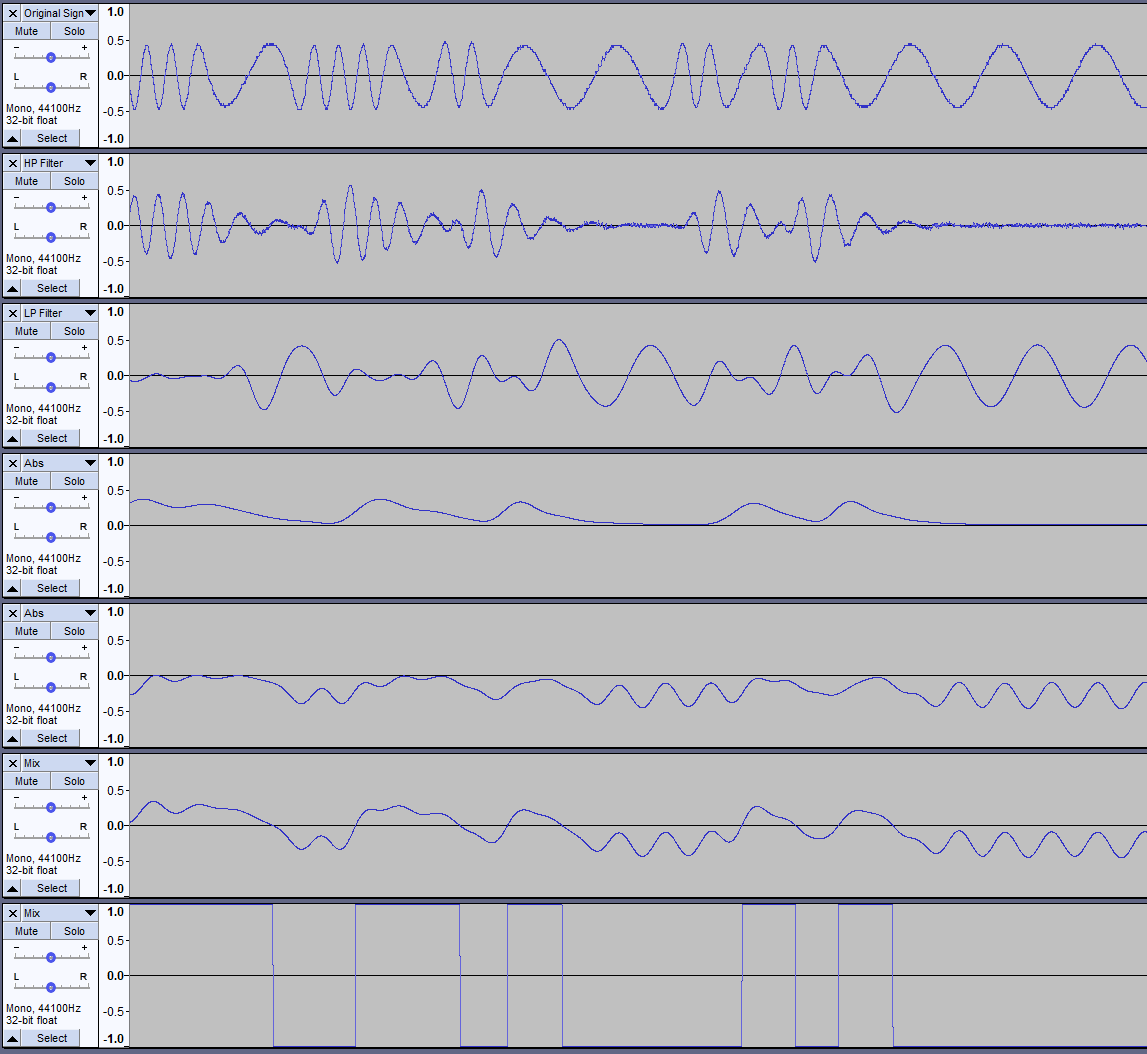
\includegraphics[width=\textwidth]{images/6-pentesting/audacity-demodulation.png}
    \caption{The process of demodulating a BFSK signal in Audacity.}
    \label{fig:audacity-demodulation}
\end{figure}
\begin{figure}[ht]
    \begin{minted}[fontsize=\footnotesize, frame=single]{python}
import matplotlib.pyplot as plt

SIGNAL_LEN, SYMBOL_LEN = 34000, 200
FILE, SIGNAL_OFFSETS = "door-signal.raw", [1800, 856160, ...]

with open(FILE, "rb") as f:
  signal = [b if b < 128 else b - 256 for b in f.read()]

for i, offset in enumerate(SIGNAL_OFFSETS):
  xs = range(offset, offset + SIGNAL_LEN, SYMBOL_LEN)
  plt.scatter(xs, [0 for _ in xs], c="red")
  bits = "".join(['1' if signal[x] > 0 else '0' for x in xs])
  print(f"Packet {str(i).ljust(2)} =", hex(int(bits, 2)))

plt.plot(signal)
plt.show()
    \end{minted}
    \caption{A program to extract bits from a binary wave and plot it.}
    \label{lst:extract-bits}
\end{figure}

\subsubsection{Results}
By using the Audacity and the method described, binary data was extracted from each recorded signal. This is presented in table \ref{tb:demodulated-data}, in hexadecimal form.
\begin{table}[!p]
    \centering
    \begin{tabularx}{\textwidth}{l}
        \hline
        \textbf{Door tamper sensor on} \\ \hline
        \texttt{0xaaaaaaaa29cd29cd0a000015d477e072b922530064} \\
        \texttt{0xaaaaaaaa29cd29cd0a0000028648b07e291d2ceecc} \\
        \texttt{0xaaaaaaaa29cd29cd0a0000280b9d2e1d2d2ca7f31c} \\
        \texttt{0xaaaaaaaa29cd29cd0a00002548c662f2feeea7fe22} \\
        \texttt{0xaaaaaaaa29cd29cd0a000019201db301398d538674} \\
        \texttt{0xaaaaaaaa29cd29cd0a00000806d6a5ee37481e2f76} \\
        \hline
        
        \textbf{Door tamper sensor off} \\ \hline
        \texttt{0xaaaaaaaa29cd29cd0a0000102366a5cb78d61c0d0c} \\
        \texttt{0xaaaaaaaa29cd29cd0a00000a3b2cb0867bf62aa616} \\
        \texttt{0xaaaaaaaa29cd29cd0a000028fe2271f089a9e8c984} \\
        \texttt{0xaaaaaaaa29cd29cd0a00001e23195bcbe8c65107ec} \\
        \texttt{0xaaaaaaaa29cd29cd0a00001913b1ee7e3448da1cf0} \\
        \texttt{0xaaaaaaaa29cd29cd0a000006f69dbb732deb2a120c} \\
        \hline
        
        \textbf{Camera tamper sensor on} \\ \hline
        \texttt{0x155555554539a539a14000034164758f44cfae66f1} \\
        \texttt{0x155555554539a539a14000034164758f44cfae66f1} \\
        \texttt{0x155555554539a539a14000034164758f44cfae66f1} \\
        \texttt{0x155555554539a539a14000034164758f44cfae66f1} \\
        \texttt{0x155555554539a539a14000034164758f44cfae66f1} \\
        \texttt{0x155555554539a539a14000034164758f44cfae66f1} \\
        \hline
        
        \textbf{Camera tamper sensor off} \\ \hline
        \texttt{0x155555554539a539a140000342724d66fce053d3d7} \\
        \texttt{0x155555554539a539a140000342724d66fce053d3d7} \\
        \texttt{0x155555554539a539a140000342724d66fce053d3d7} \\
        \texttt{0x155555554539a539a140000342724d66fce053d3d7} \\
        \texttt{0x155555554539a539a140000342724d66fce053d3d7} \\
        \texttt{0x155555554539a539a140000342724d66fce053d3d7} \\
        \hline
    \end{tabularx}
    \caption{Binary data extracted from demodulating RF signals.}
    \label{tb:demodulated-data}
\end{table}
Analyzing the data one can see a very clear structure emerging. All recorded signals decoded into exactly 170 bits and seemingly always have the following structure. See also figure \ref{fig:rf-message-structure}.
\begin{enumerate}
    \item A preamble of alternating ones and zeroes. This is a very common technique in RF protocol to notify of an incoming signal and to sync clock frequencies \cite{hacking-the-iot-talk}.
    \item A sequence of bytes that is constant for each device. E.g the door sensor will always send the same byte sequence, the camera another one, etc. This corresponds to a syncword, which is often found in RF protocols, used to determine the protocol type or from which device the message originates \cite{hacking-the-iot-talk}. Presumably, this is some kind of ID to tell the main panel from which peripheral this message is.
    \item A sequence of zero bits. Presumably, this is part of the syncword. This is also a common technique in RF protocols, to let the receiver know what protocol this is and exactly where the payload data starts \cite{hacking-the-iot-talk}.
    \item A sequence of seemingly random bits, presumably, the payload.
\end{enumerate}
\begin{figure}[!ht]
    \centering
    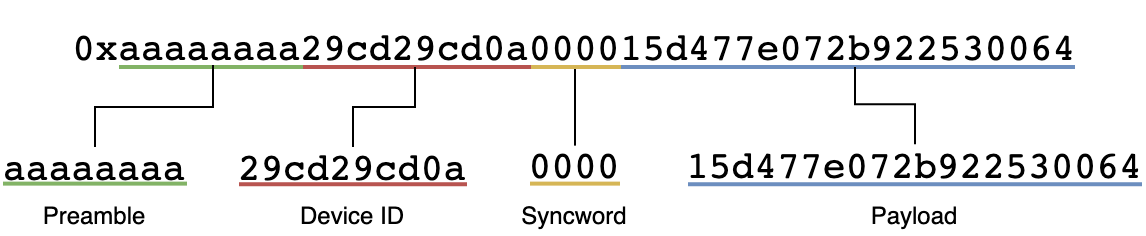
\includegraphics[width=\textwidth]{images/6-pentesting/rf-message-structure.png}
    \caption{The structure of a message in the proprietary RF protocol.}
    \label{fig:rf-message-structure}
\end{figure}
Given the final part of the message, which is seemingly random, and the fact that the replay attack presented in section \ref{ch:pentesting:replay} worked for any of the messages, we can conclude that some kind of encryption or obfuscation is used. For the tamper sensor on the door, the payload is seemingly random for every single message. For the camera sensor, however, the packets are always identical.

\subsubsection{Discussion}
The signals were successfully demodulated using the described method. Data extracted from this process shows a clear structure to the messages, giving further indication that the capturing and demodulation were done correctly. By visually inspecting the signals one could see that FSK modulation was used. Additionally, this is actually documented in the official user manual \cite{hsgw-user-manual}, meaning we can be sure that this conclusion was correct. Furthermore, the signals follow patterns and structures commonly used in RF protocols \cite{hacking-the-iot-talk}, such as starting with a preamble of alternating symbols and a syncword, which in this case seems to be some kind of ID to identify themselves in the protocol. This is discussed in section \ref{ch:related-work:hacking-iot}.

However, the payload is clearly encrypted or at least obfuscated in some way. This is in line with the documentation provided by Climax Technology, in which they reference a \enquote{Private Encryption Method} used in the RF communication \cite{hsgw-user-manual}. What the actual method is and whether or not it is a cryptographically secure method is left unanswered. It could be the case that the encryption is quite weak. Without access to the firmware or additional documentation about the RF protocol, further reverse engineering is next to impossible given the current \enquote{black box} state of the RF protocol. This means that one, unfortunately, cannot create new messages from scratch.

In conclusion, this pentest did not yield any additional actionable information. While the demodulated data definitely gives some insight into the system, it does not indicate any further vulnerabilities. Trying to reverse engineer the encryption method would yield a lot of additional information, and allow an attacker to create new messages from scratch. However, without access to the firmware, this is quite difficult and left as potential future work.
